\begin{savequote}[10cm] % this sets the width of the quote
\sffamily
Across the generations, I see that people can't get enough of each other, if and only if they can have each other at a distance, in amounts they can control. I call it the Goldilocks effect: not too close, not too far, just right.
\ldots
When I ask people ``What's wrong with having a conversation?'' People say, ``I'll tell you what's wrong with having a conversation. It takes place in real time and you can't control what you're going to say.'' So that's the bottom line. Texting, email, posting, all of these things let us present the self as we want to be. We get to edit, and that means we get to delete, and that means we get to retouch, the face, the voice, the flesh, the body -- not too little, not too much, just right.

Human relationships are rich and they're messy and they're demanding. And we clean them up with technology. And when we do, one of the things that can happen is that we sacrifice conversation for mere connection. We short-change ourselves. And over time, we seem to forget this, or we seem to stop caring.\cite{Turkle}

\qauthor{Sheree Turkle - TED 2012}
\end{savequote}

\chapter{Introduction}

\section{Abstract}
\section{Main Message}
The question in this thesis topic is broad: Can \acrfull{ict} facilitate and empower individuals and communities in Rural and Remote Australia? At once the question seems easy to answer intuitively and difficult to prove. Many branches of society believe ICT is  valuable. Successive governments in Australia have spent large sums of public money to facilitate ICT both in the provision of telecommunications networks over all sorts of technologies to the democratic provision of computer hardware and software for many Australian citizens to alleviate the gap between the digital rich and poor. The Australian Government has sponsored one of its largest national infrastructure projects ever, the \acrfull{nbn}, ``\ldots to connect Australia and bridge the digital divide, NBN’s key objective is to ensure all Australians have access to fast broadband as soon as possible, at affordable prices, and at least cost''\cite{RefWorks:459}.

Private industry too, has spent large sums of money on private networks with all the major telecommunications providers (telco's) setting up private networks based on various technology mixes. This would indicate that each of these businesses believes that owning the communications network gives them a competitive advantage in a way that sharing a common network would not.

When pressed to justify these expenses, both government and private industry resort to expected return on investment and business case arguments for providing ICT services to communities and individuals. In these cases there is always a trade off between providing a service at a cost that will ensure a payback from the user of that service. This ensures that scarce resources of everything from hardware, software and even logical resources such as radio spectrum are not allocated to a sparsely populated area with a few users and under allocated to a densely populated area with many users that over consume the resource leading to service contention.

Government and industry in Australia have been proceeding from the point of view that blanket provision of ICT is not a right of citizens beyond some minimum service levels that have existed since the telecommunications authority was in public hands. Other countries, such as Costa~Rica, Estonia, Finland, France, Greece and Spain all have requirements to give a minimum level of Internet Access to all their citizens.%reference?
 In December 2017, the UK government's telecommunications regulator, OFCOM, updated its \acrfull{uso}  to include internet access for all UK citizens as a fundamental right and expects to implement this access in some form by 2020\autocite{RefWorks:420}. While the United Nations has stopped short of so far calling access to the internet a human right, it has said that it is a human right for any such access to be free of limitation or restriction by government and that citizens should have the same rights to the internet as they have in other communications media\cite{RefWorks:421}.

\section{Approach to the question}


I originally encountered social networking as a computer science problem when I set out to investigate the Semantic Web and the way computers could encode internet based content to understand and process it. In doing so I became involved with the research of Professor Steve Cassidy at Macquarie University who's research into the semantic web had already yielded several products based around the storage and processing of texts for computer based language and learning applications.

At this stage of my research I was interested in the way Indigenous people and communities used the internet. Facebook and Twitter were new and social networking was an exciting and evolving field. I also saw that Indigenous communities were far from static and that there were many dimensions to Indigenous life that were undergoing rapid change in areas such as economics, education, fertility and location of these communities.

I looked into the area of language processing and the semantic web in Indigenous communities with the view of putting together a proposal for a multi--party Indigenous content management system that would provide a social network based mechanism for the control of media stored in it. I reasoned that, from my superficial understanding of the Indigenous social media network that there were inhibiting factors that prevented Indigenous participation in the social network that I had only recently (at that time) joined myself and that if these barriers to entry and experience were overcome, Indigenous media sharing on the internet would take off. 

I began working on a technological approach to the subject and noticed that the problems involved had largely been solved from a technical standpoint. It would be possible to implement a system that allowed Indigenous participants to encode media to any level of granularity and not only maintain control over it but monetise it so that their participation would not be exploited or repurposed in a way that misused it. One example of a similar system established for academic use is the Pacific and Regional Archive for Digital Sources in Endangered Cultures (PARADISEC)\cite{RefWorks:422}.

I found that there were many use cases that would have been thought of as singularly Indigenous which, when applied to my non-Indigenous life had direct analogues that were similar but in some ways less formally encoded because they were already part of the manners of non--Indigenous society.  Working at a television station at the time I frequently encountered examples of my own, non-Indigenous culture's  social audio-visual rights management such as a form of mortuary rights respect where advertising or documentary material that incorporated a recently deceased sports person would have to be altered to remove them or insert a dedication. Legal rights would come into play if a matter that had previously been up for discussion on a news panel needed to be suppressed on replay if that matter was now before a court or tribunal. Music frequently had to be replaced if it was found to be `copyright' music that would need to be exhibited according to the rights agreement negotiated by the television station and paid for. In many cases it was replaced with `production' music which was sold to the station for use in media that would be widely distributed and would not accrue royalties to the owner of the intellectual property.

I wondered why, when the technical issues have been solved, there was not more widespread use and continued development of the technologies that facilitate granular control of media over information technology based systems. I concluded that the solution provided by open source content management systems and media technologies such as MPEG21 and MPEG7 were not required by the market participants for these systems who were largely using open protocol systems and making as many social media faux pas as non--Indigenous counterparts. I was puzzled as to why such a useful set of technologies should be waiting on the shelves rather than being taken up by a new generation of developers such as Facebook, Google, Apple and even commercial interests who would find them a cheap and easy way to solve many of their issues around control and monetisation of media content. I theorised that these players were not using these technologies because their business models were based around strong central control of the media content management system and that technologies that promised to democratise media sharing and allow individuals to share media without strong central control would disintermediate them. Even the developer of MPEG technologies has found that so few organisations are paying to license them anymore that their business model is under threat and may collapse in the face of open source standards and software tools for creating and manipulating media\cite{RefWorks:423}.

I thought that the place of these strong central players might be taken over by free or not for profit media sharing operations in the way the open source projects such as wikipedia have managed to find a market niche but to date no project has arisen that fills this need. I was therefore drawn to consider some of the reasons that a technological solution to this problem has not succeeded so far.

The more research I did into a technical solution to the issues that prevented Indigenous social networks from being successful, the more I found that there were external factors that would need to change before such a network would be valuable and ubiquitous in those communities. 


\section{Methodology}
I investigated a pure anthropological approach to the subject of social media in remote communities but I felt that this left out other necessary areas and considered the actors in the communities to be relatively powerless. Well meaning individuals are certainly paying attention to IT use in remote communities and facilitating this use as a means to providing for a community that is perceived to be small, remote and disadvantaged. 

I felt that I was drawing from so many different areas to answer what had begun as a purely technological question that I found it hard to frame a way of investigating the problem and learning where a solution might take hold. I felt that another issue for the non-urban communities is that, as well as experiencing rapid technological change they are experiencing a shift in its constitution from average to lower than average incomes\cite{RefWorks:424}, from disconnected and personal interactions that happen between individuals in local communities to the connected and impersonal interactions that occur when these communities are connected to urban communities via the internet, mobile phone and satellite communications or via  improved transportation networks. 

I explored different anthropological and social research methodologies that described technology change over time and determined that I required a framework to bound and guide my research on this thesis topic. I decided to examine the basic dimensions of people's lives around their economic well being and their health and well being and how cultural and social systems interact with them.

I was attracted to this theory of social economics and change management due to its consideration of exogenous factors in moving from one technology to another. A common element in the story of failure of many Community initiatives is their failure to consider any of the influences external to the change that the program is set up to promote in the community. In the complex social and cultural systems of rural and remote communities, these influences are almost certain to undermine any technology change initiative due to their lack of support and consideration of, the cultural and social environment. Change projects that involve technology implementations are especially susceptible to failure  through failure to consider stakeholder influence and requirements.\cite[23-24]{RefWorks:115}  I was also confronted by the speed of change in the technology platforms under evaluation for a target media management system that I had intended to design at the earliest stage of my thesis project. I found that the technology was moving on rapidly and I needed a way to accommodate the end state technology for an implementation that was several years away, not the technology platform that existed in the environment in remote and regional Australia at the time of writing.







\section{Research Objective- - Survey}
This survey was devised to ascertain the quality of internet access across a range of locations and the effect of the internet on the dimensions of experience that are relevant to this thesis, namely Health and Well-being, Culture and Society and participation in the Economy. 
\section{Hypothesis}
My assumption was that access to the internet and the quality of that access made and makes a material difference to the quality of life of those people who can access it in the five dimensions of cultural and social interaction and participation, health and emotional well-being and economic well-being.
\section{Methods}
The survey was conducted by commissioning an organisation, \index{Qualtrics} Qualtrics, to administer the survey with certain parameters. This organisation was selected as it was one that is already used by Macquarie University for survey tools for social science surveys and because they have recently started recruiting general purpose Australian survey panels having opened an office in Australia. Qualtrics paid participants for completing their surveys according to their agreement with them. Funding was limited to \$5,000 which was obtained through a research grant made available by the Department of Computer Science at Macquarie University. The survey was administered in five regions denoted by Australian Bureau of Statistics (ABS) remoteness categories: Major Cities of Australia (MCA), Inner Regional Areas (IRA), Outer Regional Areas (ORA), Remote Areas of Australia (RA) and Very Remote Areas of Australia (VRA). I decided to use these areas to correlate results from this survey with similar results from the ABS in the same regional areas. These areas were determined by the respondent identifying their postcode which the ABS had already classified according to these remoteness characteristics. In some cases the respondent may have a different postcode to the GPS coordinates of the internet location at which they lodged the survey. This may be due to their need to go from a remote or very remote area to obtain internet services to undertake the survey.

Qualtrics maintains panels that respond to surveys internationally. Some initial valid responses were made outside of Australia and these results were rejected. They may have been from Australians who were travelling and filling out the survey from an international location but the it was also possible that they were done by `gold mining' overseas workers who were filling out many surveys for material gain and so these results were rejected. 

It was relatively easy to obtain a large response in Major cities and Regional Areas and a quota of one hundred responses was set for Major Cities, Inner Regional and Outer Regional areas in Australia and thirty-five each for Remote and Very Remote Australian populations. In practice it was difficult to collect a large sample from Remote and Very Remote areas. This was due to budget limitations with collecting these respondents and with the lack of people on the Qualtrics panel who could respond to the survey on the internet. Qualtrics could have supplied more respondents for each population if the budget had been larger. Unfortunately, implementation coincided with a currency movement which adversely affected Australian/US Dollar exchange rate and this meant the survey size was reduced from a proposal for over 450 respondents to one of 345 respondents to stay within the budget of \$5,000 Australian Dollars which cost \$3,780 US Dollars at the time of the survey. A proposal for one thousand participants which would have had three hundred respondents in Major Cities, Inner and Outer Regional Australia and fifty each in Remote and Very Remote Australia was proposed at a cost of \$12,838 Australian Dollars. This may be an avenue for future comparative research in the area to contrast these results for the same regions at a future date.

In all, 1,682 responses were started but only 345 answered the mandatory questions and met the demographic criteria. Mandatory criteria were:
\begin{enumerate}[(a)]
\item Must be over the age of 18
\item Must be completing the survey from a device with an Australian postcode
\item Must be completing the survey from a device that is geo-located on the Australian mainland
\end{enumerate}

100 respondents were found in Major Cities and Inner and Outer Regional Areas but only 35 qualified respondents were found in the Remote Areas and only 10 respondents in Very Remote Areas.

The time required to complete the survey was judged to be under 15 minutes by the Qualtrics automatic survey test. The survey had 50 questions divided into six sections according to the dimensions being researched in the thesis. The survey was available on the Qualtrics portal for five weeks between 20 July 2016 and 28 August 2016. Specific attention was paid to making the survey viewable on mobile devices as the use of mobile devices such as phones and tablets was a focus area of the research.

Analysis of the results was conducted with Microsoft Excel and scripts run in the R language. 


\section{Data Analysis}
Data was analysed using R to produce violin plots to show how groups in the different populations cluster together. These plots show frequency and amplitude of responses to questions that have multiple dimensions such as the number of people spending more than \$50 on internet use in Very Remote Areas of Australia. Quantitative information that only involved one dimension, the number of people using wired or wireless connections, for example, were analysed with Microsoft Excel Pivot Tables and charted with either Microsoft Excel or the \LaTeX ~tikz library to produce ring plots.


\section{Main Findings}
\subsection{Demographics}
\begin{figure}
\centering
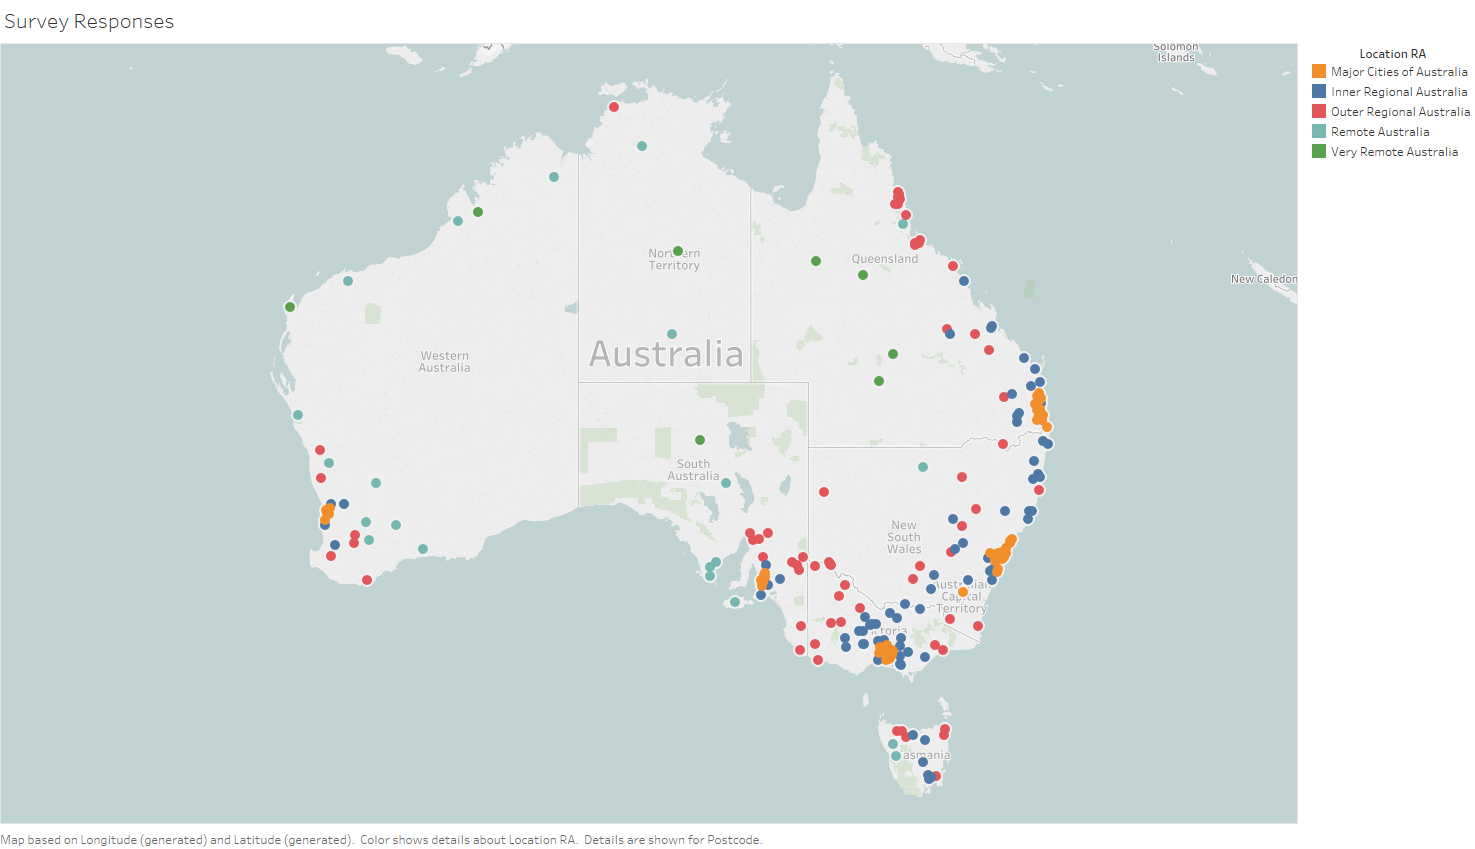
\includegraphics[scale=0.40]{figures/SurveyResponses.png} 
\caption{Locations of Responses}
\label{fig:ResponsesMap}
\end{figure}
Respondents came from all states and territories. While on the map, Figure~\ref{fig:ResponsesMap}, it appears that respondents are clustered around capital cities, this is a function of the scale of the map.



\begin{figure}
\centering
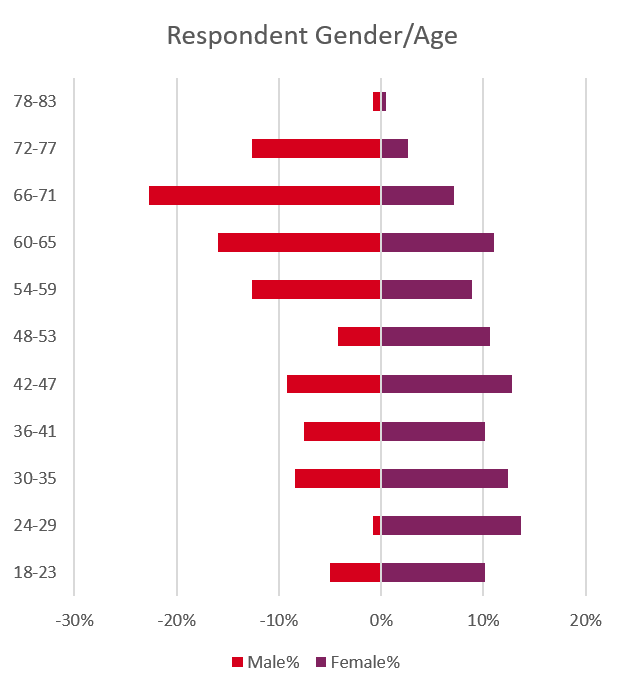
\includegraphics[scale=0.5]{figures/ResponseGender.png} 
\caption{Age and Gender of Respondents}
\label{fig:ResponseGender}
\end{figure}
Figure~\ref{fig:ResponseGender} shows a population pyramid of the age and gender of Respondents. A relatively uniform number of female respondents are seen through almost all age groups, rarely dropping below 10 percent while the age of the male respondents is highly variable and climbs to over double the average of female respondents when the male respondents approach and reach retirement age of 65 before dropping back over 72 years old. This behaviour seems to indicate that women from all age groups were predisposed to take survey this survey but that only men around the age of retirement were. 

\subsection{Technology}
The majority of respondents used the Windows operating system to respond and the majority of those systems were running the latest version of the system, Windows~10. 
\begin{figure}
\centering
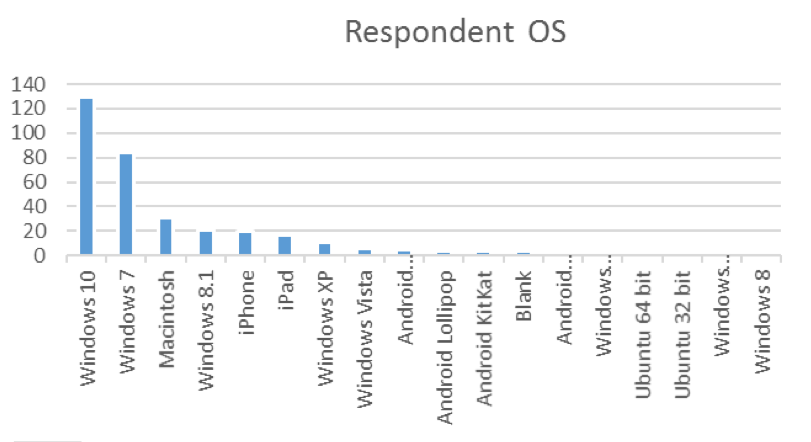
\includegraphics[scale=1]{figures/Survey-OS.png} 
\caption{Operating Systems used by Respondents}
\label{fig:surveyOS}
\end{figure}
Of these respondents, most were using desk-bound computers and majority of these were running the most recent Microsoft Windows operating system, version 10. This information was taken from metadata the browser reported to the survey website. This indicated that very few mobile devices were being used to respond to the survey as there were very few iOS Safari or Android operating systems present in the response data. A very small number of Linux machines were seen in the data but fewer Apple Macintosh systems were found than expected. 



